%!TEX root = ../Bachelorseminar-RoboticSwarms.tex

	\begin{center}
		\def\loclb{(180:2.0cm) circle (2.0cm)}
	  	\def\loclf{(0:2.0cm) circle (2.0cm)}
	  	\def\locrb{(90:2.0cm) circle (2.0cm)}
	  	\def\locrf{(270:2.0cm) circle (2.0cm)}

	    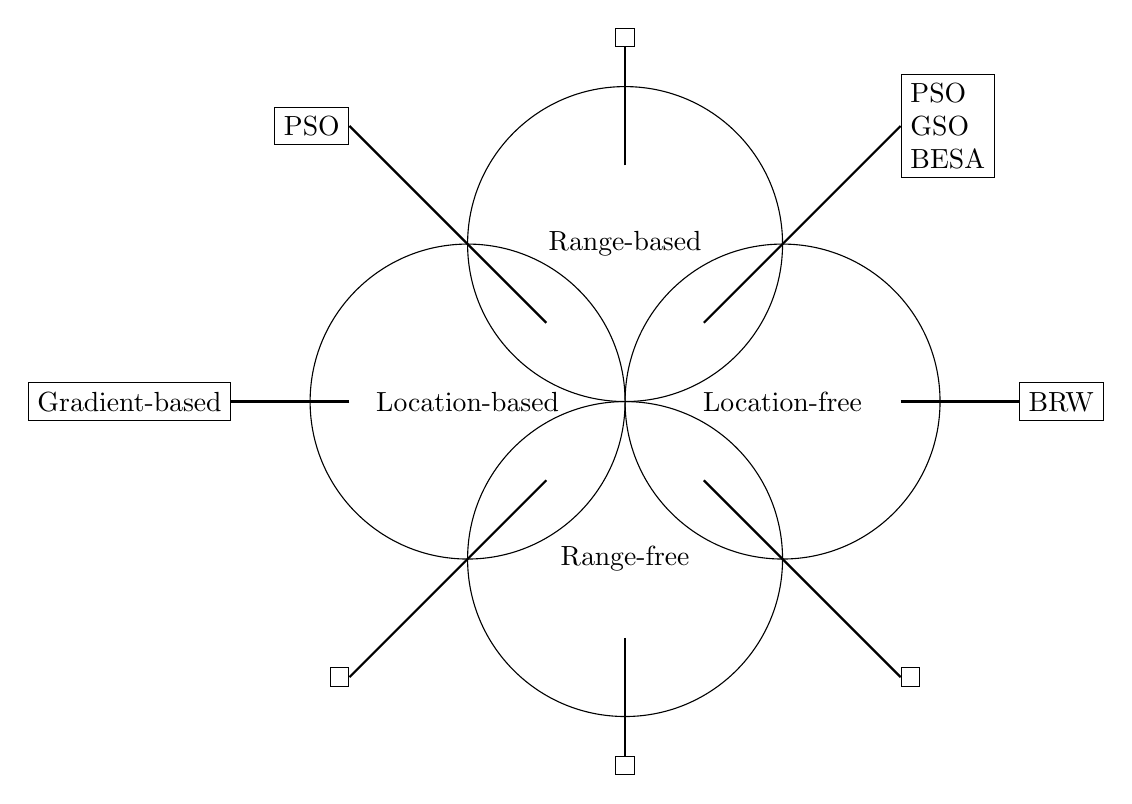
\begin{tikzpicture}
			% standard figures
			\draw \loclb node [text=black] {Location-based};
			\draw \loclf node [text=black] {Location-free};
			\draw \locrb node [text=black] {Range-based};
			\draw \locrf node [text=black] {Range-free};

			% Range-based localization-free
			\draw[thick,-] (1,1) -- (3.5,3.5) node[anchor=north west] {};
			\node[draw,align=left,anchor=west] at (3.5,3.5) {PSO\\GSO\\BESA};

			% Range-free, localization-free
			\draw[thick,-] (1,-1) -- (3.5,-3.5) node[anchor=north west] {};
			\node[draw,align=left,anchor=west] at (3.5,-3.5) {};

			% Localization-free
			\draw[thick,-] (3.5,0) -- (5,0) node[anchor=north west] {};
			\node[draw,align=left,anchor=west] at (5,0) {BRW};

			% Localization-based
			\draw[thick,-] (-3.5,0) -- (-5,0) node[anchor=north west] {};
			\node[draw,align=left,anchor=east] at (-5,0) {Gradient-based};

			% Range-free, localization-based
			\draw[thick,-] (-1,-1) -- (-3.5,-3.5) node[anchor=north west] {};
			\node[draw,align=left,anchor=east] at (-3.5,-3.5) {};

			% Range-based, localization-based
			\draw[thick,-] (-1,1) -- (-3.5,3.5) node[anchor=north west] {};
			\node[draw,align=left,anchor=east] at (-3.5,3.5) {PSO};

			% Range-based
			\draw[thick,-] (0,3) -- (0,4.5) node[anchor=north west] {};
			\node[draw,align=left,anchor=south] at (0,4.5) {};

			% Range-free
			\draw[thick,-] (0,-3) -- (0,-4.5) node[anchor=north west] {};
			\node[draw,align=left,anchor=north] at (0,-4.5) {};
		\end{tikzpicture}
    \end{center}